 
 
\documentclass[12pt]{article}

\usepackage{fullpage}
\usepackage{multicol,multirow}
\usepackage{tabularx}
\usepackage{ulem}
\usepackage[utf8]{inputenc}
\usepackage[russian]{babel}
\usepackage{graphicx}

\usepackage{float}

\begin{document}

\section*{Лабораторная работа №\,5 по курсу дискртного анализа: Суффиксные деревья
}

Выполнил студент группы 08-208 МАИ \textit{Куликов Алексей}.

\subsection*{Условие}

Необходимо реализовать алгоритм Укконена построения суффиксного дерева за линейное время для алфавита строк: строчные буквы латинского алфавита (т.е., от a до z). 
Далее, построив такое дерево для некоторых из входных строк, необходимо воспользоваться полученным суффиксным деревом для поиска образца с использованием статистики совпадений.

\subsection*{Метод решения}

В данной реализации суффиксное дерево строится при помощи алгоритма Укконена с использованием active-point. Active-point -- три переменные, задающие текущее положение в суффиксном дереве, от которого будут производиться дальнейшие сравнения и в которое будут (при необходимости) вставляться новые вершины.

Active-point состоит из:
\begin{itemize}
    \item Active-node -- узел, из которого будет выбираться исходящее ребро.
    \item Active-edge -- символ в начале выбираемого ребра, необходимый, собственно, для его выбора.
     \item Active-length -- задает позицию в рамках выбранного ребра.
\end{itemize}

Вместо подстрок исходной строки в явном виде, будем хранить в качестве метки ребра пару индексов $[l, r]$, где $l$ -- индекс левой границы подстроки, $r$ - индекс правой границы подстроки.

Построение суффиксного дерева для заданной строки делится на $m$ фаз. Каждая $i$-тая фаза делится в свою очередь на $i-1$ продолжений. Каждое из продолжений имеет один из 3-х видов:

\begin{enumerate}
    \item Путь для текущего продолжения кончается в листе. Тогда просто продлеваем метку для этого листа на один символ. В данной реализации все продолжения такого типа будут совершаться за $O(1)$ действий простым увеличением значения переменной, хранящей индекс конца каждого из существующих листов.
    \item Путь для текущего продолжения оканчивается во внутренней вершине либо посередине ребра. В данном случае явной вставки не избежать. 
    
    Если путь закончился во внутренней вершине, то просто добавляем новое исходящеее ребро в лист дерева, помеченное меткой $[i, end]$, где $i$ -- номер текущей фазы, $end$ -- та самая глобальная переменная, храянящая индекс конца.
    
    Если же путь закончился посередине ребра, то нужно вставить в этом месте новую внутреннюю вершину и добавить исходящее ребро в новый лист, как сказано выше.
    \item
    Если при попытке продолжения пути оказалось, что следующий символ уже в дереве представлен далее, то не делаем ничего. В данной реализации просто завершаем фазу.
\end{enumerate}

В конце каждого продолжения осуществляется переход к следующему суффиксу:

Если текущая активная вершина не является корнем, то переходим по суффиксной ссылке, иначе инкрементируем индекс, отвечающий за выбор ребра в начале каждого продолжения, и декрементируем пройденную длину от корня.

Это позволяет избежать наивного спуска от корня во время каждого продолжения и, как следствие ускоряет алгоритм.

Построение статистики совпадений для текста осуществляется с помощью суффиксного дерева.

Суть алгоритма в следующем. 
Идем, сравнивая символы из текста и меток проходимых ребер суффиксного дерева, до первого несовпадения. Т.о. максимально углубившись достигаем какой-то точки, в которой дальнейшее совпадение невозможно либо из-за того, что нету нужного символа, либо из-за того, что пришли в лист. 

Теперь записываем в вектор-результат $ind$ индекс в тексте, до которого продвинулись.

Если эта точка -- внутренняя вершина, то переходим по суффиксной ссылке. Если же остановились посередине ребра или в листе, то поднимаемся вверх до первой внутренней вершины, переходим по суффиксной ссылке.

Если останавливаемся на ребре, смежном с корнем дерева, то начинаем в следующей итерации сравнивать от корня.

Далее начинаем сравнивать с позиции, которую достигли в прошлом суффиксе, только для суффикса короче на 1 символ. Проделав сравнения и опять остановившись по какой-то причине, пишем в вектор индекс $ind - 1$ т.к. этот суффикс короче на 1.

И так далее.

Если в какой-то момент оказалось, что не моем выйти из корня из-за отсутствия ребра, помеченного текущим символом в тексте, то просто записываем результат на единицу меньший чем в прошлой ячейке и переходим к поиску для следующего символа текста.

Если в какой-то момент $ind$ достигнет длины текста, то дальнейшие явные сравнения бессмысленны. Значения оставших ячеек будут уменьшаться с каждым шагом.

\subsection*{Описание программы}

Программа состоит из единственного файла. В нем определен класс \verb|TSuffTree|, реализующий функционал суффиксного дерева (частично). Класс реализует конструктор, в котором и заключается построение суффиксного дерева, различные вспомогательные методы, вложенную структуру для представления узлов суффиксных деревьев и деструктор. Так же отдельным методом выделен \verb|getMatchStatistic|, строящий для переданного в него текста статистику совпадений.

\subsection*{Дневник отладки}

\begin{enumerate}
\item 19.02 - 3.03. В процессе разработки возникают трудности с пониманием алгоритма (как выяснилось, мелких деталей).
РЕШЕНИЕ: поиск информации, чтение, пробы и ошибки.

\item 4.03. Запутался окончательно, код стал нечитаемым из-за нагромождения условий, которые (как я думал) должны учесть все не стандартные случаи.
РЕШЕНИЕ: начать с нуля.

\item 6.03. Не отрабатывает прыжок по счетчику. Затруднения с написанием этого кусочка программы используя \verb|activeEdge| символ.
РЕШЕНИЕ: в \verb|activeEdge| хранить не символ для перехода, а индекс, по которому в строке лежит нужный символ.

\item 9.03. \verb|walkdown| не должен работать сплошняком. Он не учитывает ситуацию, когда после прыжка \verb|activeLen| становится 0.
РЕШЕНИЕ: сделал его раздельным, <<давая шанс>> блоку кода с проверкой \verb|activeLen| на 0.

\item 14.03. Суффиксное дерево запустилось окончательно. Начинаем статистику совпадений.
РЕШЕНИЕ: изучение.

\item 18.03. История с запутыванием повторяется.
РЕШЕНИЕ: статистику с нуля.

\item 20.03. В общем случае работает, но падает на частных данных. Пошаговая отладка в IDE.
РЕШЕНИЕ: оказывается алгоритм в сравнении доходит до конца строки-текста и после принимает некорректное состояние. Пришел к мысли, что если дошел до конца, то все незаполненые можно заполниить без явного обхода и закончить алгоритм.

\item 24.03. Для тестирования написал наивный алгоритм и сравнил ответы. Они не совпадают. При этом наивный правильный.
РЕШЕНИЕ: оказывается все это время при построении суффиксного дерева не правильно выставлялись суффиксные ссылки, при этом дерево строилось правильно. Исправил логику добавления СС из вершинвы с прошлого продолжения в текущую.
 
\end{enumerate}

\subsection*{Тест производительности}

Ниже приведены некоторые данные, касающиеся производительности реализованного суффиксного дерева и алгоритма построения статистики совпадений.

\begin{figure}[H]
  \caption{Зависимость времени работы алгоритма построения суффиксного дерева от длины паттерна}
  \centering
       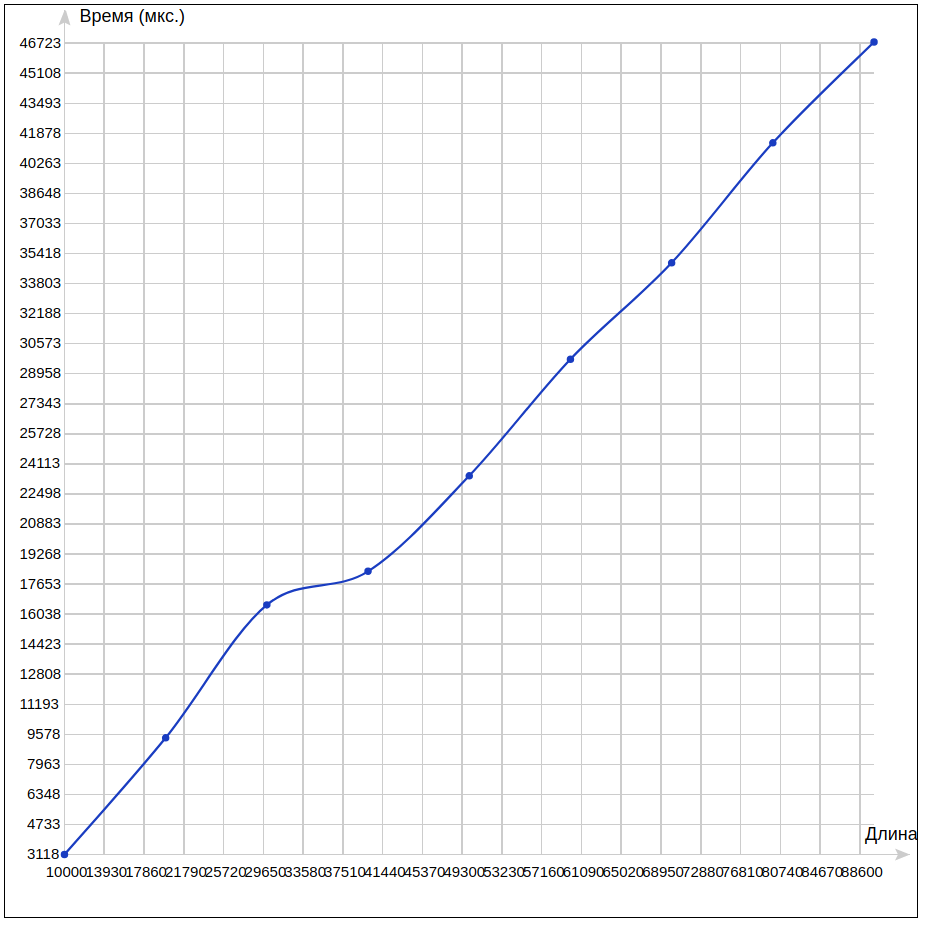
\includegraphics[width=\linewidth]{st.png}
\end{figure}

\begin{table}[h]
\caption{Время построения суффиксного дерева}
\label{tabular:timesandtenses}
\begin{center}
\begin{tabular}{|l|c|}
\hline
\textbf{Длина образца} & \textbf{Время работы (мкс.)} \\
\hline
100 & 23 \\
\hline
1000 & 153 \\
\hline
10000 & 3033 \\
\hline
100000 & 58450 \\
\hline
\end{tabular}
\end{center}
\end{table}

% построение суффиксного дерева 
% (100;23)
% (1000;153)
% (10000;3033)
% (100000;58450)

При замерах производительности для статистики совпадений был взят фиксированный паттерн длины 100.

\begin{figure}[H]
  \caption{Зависимость времени работы алгоритма построения статистики совпадений от длины текста)}
  \centering
       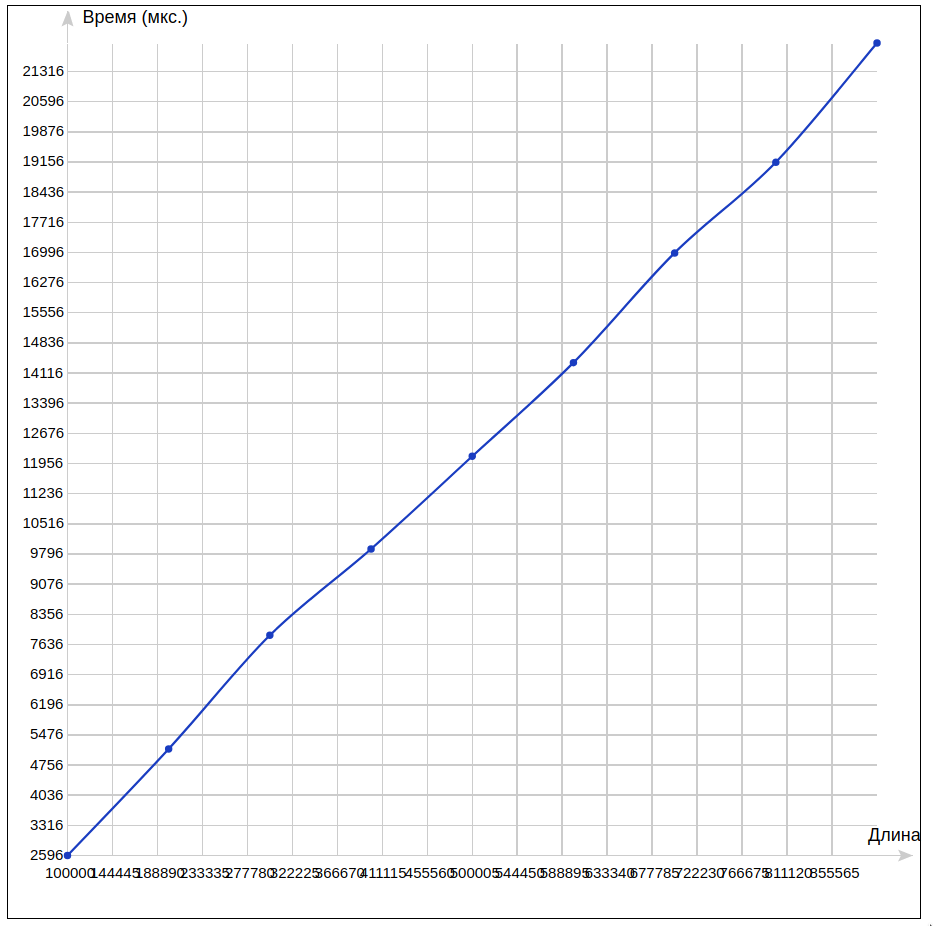
\includegraphics[width=\linewidth]{ms.png}
\end{figure}

\begin{table}[h]
\caption{Время построения статистики совпадений}
\label{tabular:timesandtenses}
\begin{center}
\begin{tabular}{|l|c|}
\hline
\textbf{Длина текста} & \textbf{Время работы (мкс.)} \\
\hline
1000 & 44 \\
\hline
10000 & 310 \\
\hline
100000 & 2980 \\
\hline
1000000 & 23270 \\
\hline
10000000 & 280470 \\
\hline
\end{tabular}
\end{center}
\end{table}

% построение статистики совпадений паттерн 100 

Из графиков зависимостей можно видеть, что время работы местами незначительно откланяется от линейной зависимости. Этого мы и хотели добиться.

\subsection*{Недочёты}

Важным недочетом является то, что структура данных, используемая для узлов дерева статична и после создания всегда занимает память под указатели, количество которых равно мощности используемого алфавита. Здесь более удачным выбором оказался бы \verb|std::map|, потому что если считать алфавит фиксированным и довольно небольшим, то время доступа к элементу достаточно мало и большой роли не сыграет. Куда важнее количество памяти.

Так же, если совсем заморочиться, можно средствами ООП избавиться от лишней занимаемой памяти. Например, для листовых узлов дерева суффиксная ссылка всегда пустует, а это 8 байт памяти на штуку. При том, листьев всегда значительно больше, чем внутренних вершин.

Вобщем, есть к чему стремиться.

\subsection*{Выводы}

Суффиксное дерево довольно мощная структура данных, имеющая множество приложений в задачах обработки строк. Среди них нахождение включения одной строки в текст, поиск наибольшей общей подстроки для набора строк, и т.д . Так же суффиксное дерево является вспомогательным, например, при построении суффиксных массивов, поиске статистики совпадений и скорее всего где-нибудь еще.

Написание суффиксного дерева мне показалось довольно сложным занятием.
Мало того, что алгоритм сам по себе не очень простой, но, даже если разобраться на бумаге и начать писать с нуля, то приходишь к выводу, что в этом алгоритме очень много мелких деталей. Неправильно поняв(закодив) одну из них суффиксное дерево отказывается запускаться либо совсем, либо ломается на частных данных.

\end{document}

